
%=============================================================================

\section{Kurvendiskussion}
\label{sec:kurvendiskussion}

Autor: Andreas Zöllner

\noindent "Uberarbeitung: Gerhard Gossen

\mbox{}\par

\noindent Eine Kurvendiskussion hilft uns eine Funktion zu "`verstehen"'. Wir bekommen Informationen über die Form des Graphs (z.~B. Anzahl und Lage von Extrema und Wendepunkten) und über wichtige Punkte (z.B. Nullstellen) der Funktion.

\noindent Eine Kurvendiskussion hat eine feste Reihenfolge von Schritten. Einige davon können von Mathematik-Programmen durchgeführt werden, aber bei komplexeren Funktionen ist der eigene Hirnschmalz gefragt.

\subsection{Definitionsbereich}

Als erstes sollte man sich über den Definitionsbereich $D(f)$ der Funktion $f$
im Klaren sein: Für welche Werte $x\in\real$ ist $f(x)$ überhaupt definiert? Die Funktion $\frac{1}{x-1}$ ist beispielsweise für $x=1$ nicht definiert (Division durch 0!), die Logarithmusfunktion ist nur für positive Werte definiert. 

\noindent Isolierte Punkte, an denen $f$ nicht definiert ist, heißen
\textbf{Definitionslücken}. Hierbei unterscheidet man verschiedene Arten von
Definitionslücken, worauf wir hier jedoch nicht näher eingehen wollen.

\noindent Der Definitionsbereich wird als Menge angegeben. Beispiele für verschiedene Bereich gibt Tabelle~\ref{tab:definitionsbereiche}.

\begin{table}[b]
\begin{tabular}{l|p{13em}}
\textbf{Definitonsbereich} & \textbf{Beschreibung}\\
\hline
$D(f) = \R$ & Der Definitionsbereich ist die gesammte Definitionsmenge.\\

$D(f) = \R \setminus \{c\}$ & Die Funktion hat eine Definitionslücke an der Stelle $c$.\\
$D(f) = \{x\in\R\ |\ a < x < b \wedge x\geq c\}$ & $f$ ist nur in den Intervallen $(a,b)$ und $[c,\infty)$ definiert.
\end{tabular}
\vspace{-1em}
\caption{Beispiele für Definitionsbereiche}
\label{tab:definitionsbereiche}
\end{table}



%=============================================================================

\subsection{Wertebereich}

Der Wertebereich einer Funktion lässt sich meist über Betrachtungen zur
Stetigkeit, der Extrema, der Monotonie und der Asymptoten ermitteln.


%=============================================================================

\subsection{Nullstellen}

Eine Stelle $x_0\in{}D(f)$ heißt eine \textbf{Nullstelle} der Funktion $f$,
wenn
\[
f(x_0)
\ =\ 0
\,,
\]
zur Bestimmung der Nullstellen müssen wir daher alle Lösungen der Gleichung \[f(x)\ =\ 0 \] finden.

%=============================================================================

\subsection{Extrema}

Um die Extrema einer Funktion $f$ bestimmen zu können, müssen die ersten beiden Ableitungen von $f$ existieren. Eine Stelle $x_0$ ist ein Extremum von $f$, wenn gilt:
\begin{enumerate}
\item $f'(x_0) = 0$ (\emph{notwendige Bedingung}) 
\item $f''(x_0) \neq 0$ (\emph{hinreichende Bedingung})
\end{enumerate}

\noindent Bei $f''(x)>0$ liegt ein lokales Minimum, bei $f''(x)<0$ ein lokales Maximum vor.
\newline \newline
\noindent Die \textbf{globalen Extrema} erhält man, indem man zusätzlich das Verhalten der
Funktion an den Grenzen des Definitionsbereichs in Betracht zieht. Also z.\,B.
falls $D(f)=\real$ sind dies die Werte $\lim_{x\to\pm\infty}f(x)$.
\newline \newline
\noindent Die erste Ableitung gibt also die Steigung der Tangenten an den Graphen an. Links von einem Maximum ist die Steigung positiv, rechts davon ist sie negativ (siehe Abb.~\ref{fig:tangenten}). Der Nulldurchgang der Ableitung entspricht also einer Tangenten mit der Steigung $0$, also einer horizontalen Gerade. Bei einem Minimum wechselt die Steigung der Tangenten entsprechend von negativ zu positiv.

\begin{figure}
\begin{center}
    \begin{minipage}[b]{.4\textwidth}
    \begin{center}
        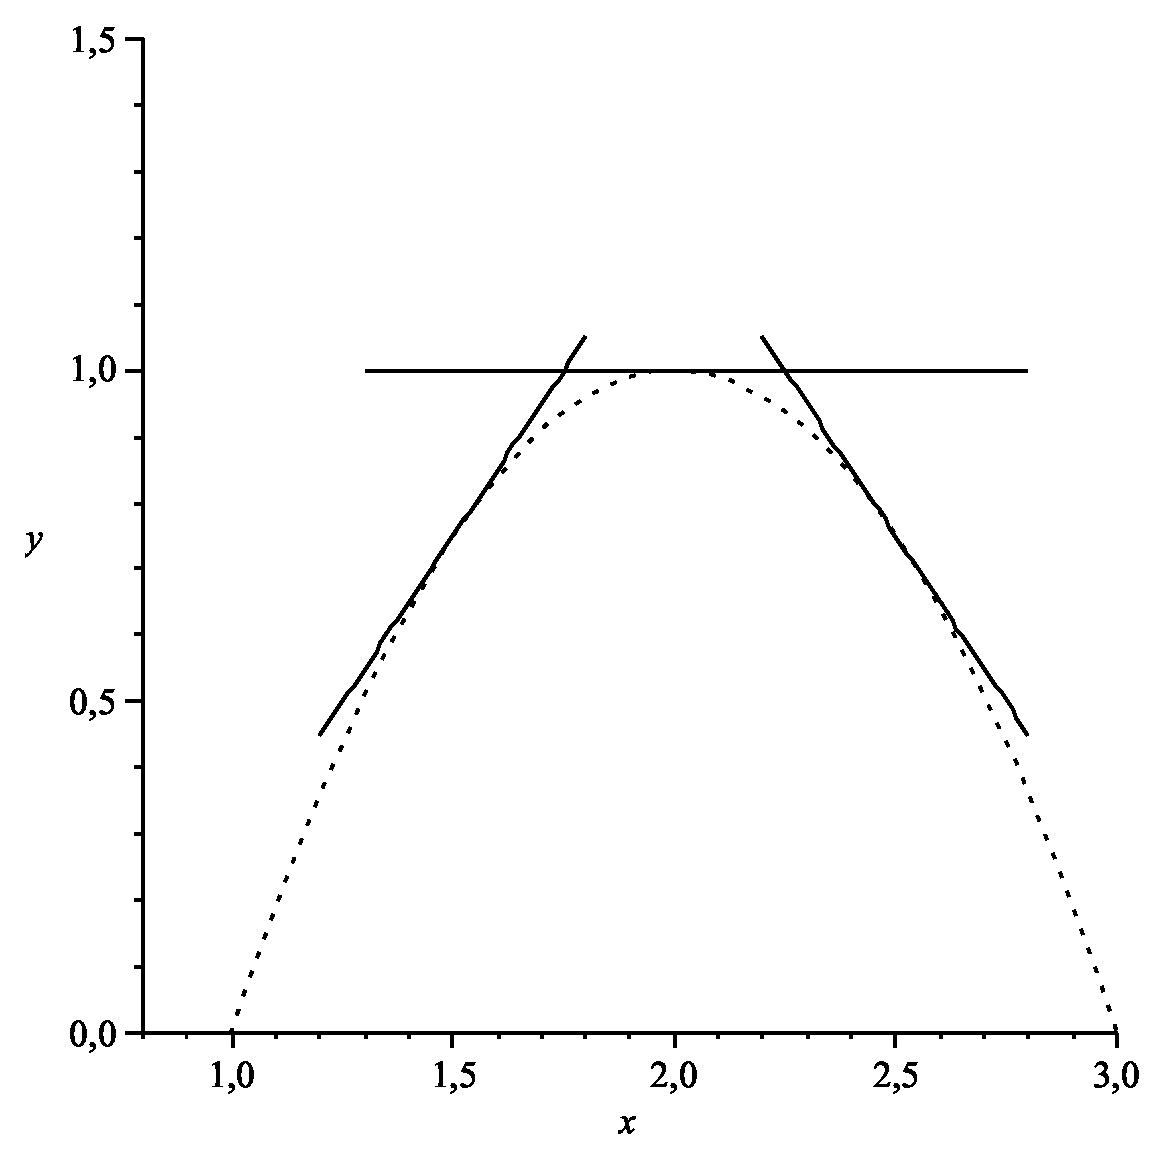
\includegraphics[width=.8\textwidth]{img/tangenten}
    \end{center}
    \caption{Tangenten der Funktion $-(x-2)^2+1$ an den Stellen $\frac{3}{2},2, \frac{5}{2}$}
    \label{fig:tangenten}
    \end{minipage}
    \hspace{.1\textwidth}
    \begin{minipage}[b]{.41\textwidth}
    \begin{center}
        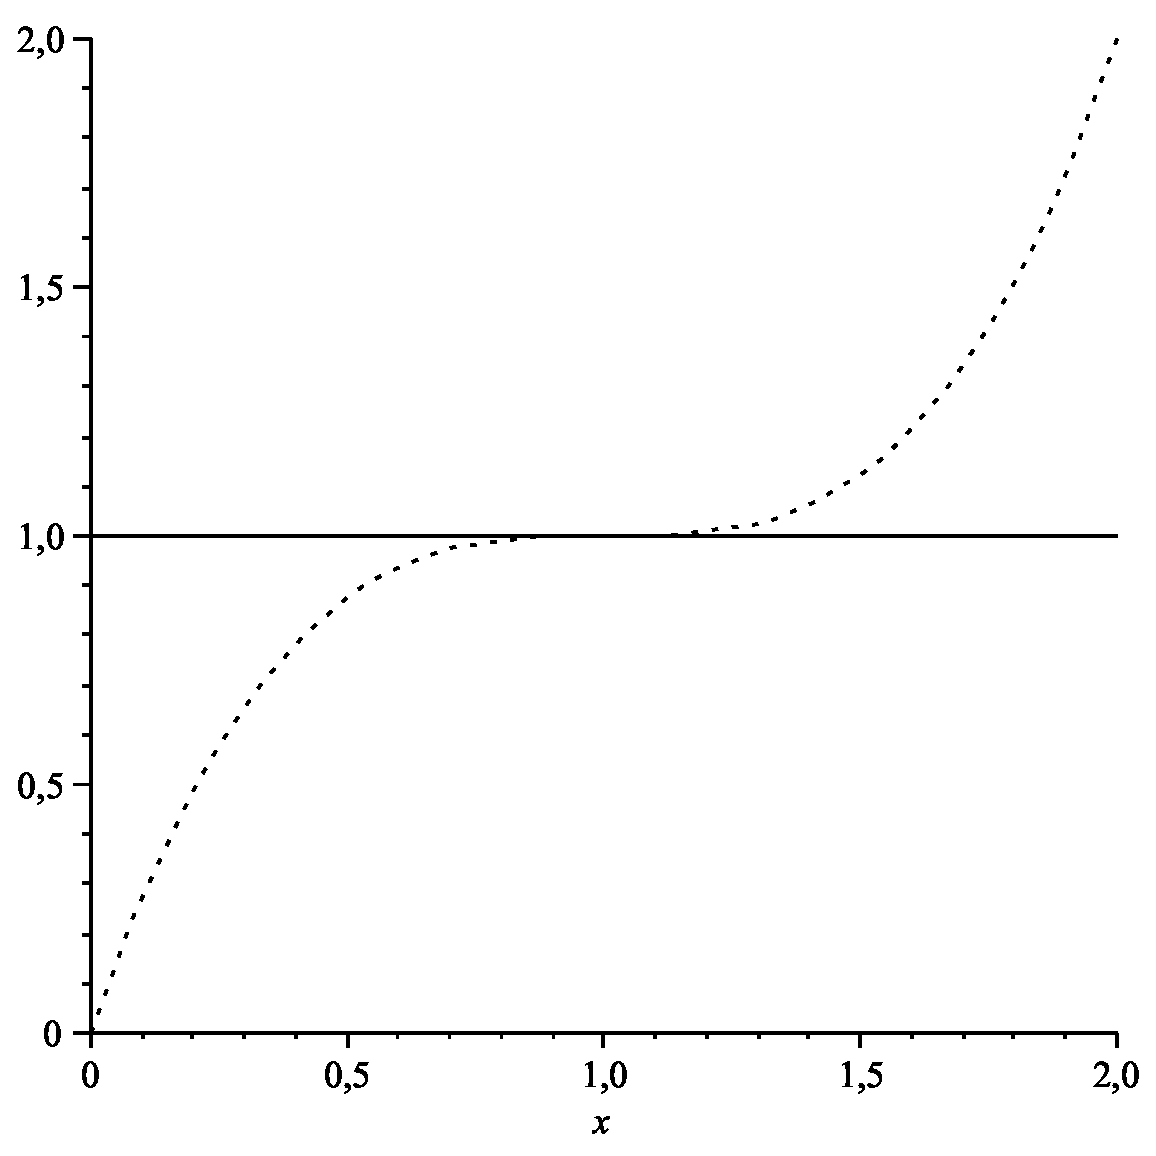
\includegraphics[width=.8\textwidth]{img/sattelpunkt}
    \end{center}

    \caption{Sattelpunkt der Funktion $(x-1)^3+1$ an der Stelle $x=1$}
    \label{fig:sattelpunkt}
    \end{minipage}
\end{center}

\end{figure}
%%%%%%%%%%%%%%%%%%%%%%%%%%%%%%%%%%%%%%%%%%%%%%%%%%%%%%%%%5
\newpage
\subsection{Exkursion: Ableiten einer Funktion} 
%\label{sec:ableitungen}
\subsubsection{Differentiationsregeln}
\begin{enumerate}
\item Faktorregel: $c\cdot f(x)(c \in \mathbb{R},konstant) \Rightarrow c\cdot f'(x)$
\item Summenregel: $f(x) + g(x) \Rightarrow f'(x)+g'(x)$
\item Produktregel:$f(x)\cdot g(x) \Rightarrow f'(x)\cdot g(x) + f(x)\cdot g'(x)$
\item Quotientenregel: $\displaystyle \frac{f(x)}{g(x)} (g(x)\neq 0) \Rightarrow \displaystyle \frac{f'(x)g(x) - f(x)g'(x)}{(g(x))^2}$
\item Kettenregel: $f(g(x)) \Rightarrow f'(g(x))\cdot g'(x)$
\end{enumerate}

\subsubsection{wichtige Ableitungen}
\begin{center}
\begin{tabular}{c|c}
Funktion & Ableitung\\
\hline
$c$ & $0$\\
$x^n$ & $n\cdot x^{n-1}$\\
$sin x$ & $\cos x$\\
$cos x$ &$-\sin x$\\
$tan x $& $\displaystyle \frac{1}{\cos^2 x}$\\
$e^x$ & $e^x$\\
$ln x$ & $\frac{1}{x}$\\
\end{tabular}
\end{center}
%%%%%%%%%%%%%%%%%%%%%%%%%%%%%%%%%%%%%%%%%%%%%%%%%%%%%%
\subsection{Wendepunkte}

An einem \emph{Wendepunkt} ändert sich das Krümmungsverhalten des Funktionsgraphen, der Graph wechselt also von einer Links- in eine Rechtskurve oder umgekehrt.

\noindent Das notwendige Kriterium für eine Wendestelle bei $x_0$ ist, dass der Wert der zweiten Ableitung Null wird: $f''(x_0) = 0$. Zusätzlich muss noch eine der beiden folgenden Bedingungen erfüllt sein:
\begin{description}
    \item[Der Wert der dritten Ableitung ist ungleich Null:] $f'''(x_0)\neq 0$. Dabei muss aber die dritte Ableitung existieren.
    \item[Das Vorzeichen der zweiten Ableitung wechselt in $x_0$:] Falls keine dritte Ableitung existiert oder ihre Berechnung zu aufwändig ist, muss man das Vorzeichen auf beiden Seiten von $x_0$ vergleichen.
\end{description}

\noindent Die zweite Ableitung gibt die Änderung der Steigung an. Wenn die zweite Ableitung positiv ist, wird die Steigung größer, der Graph macht also eine Linkskurve. Eine Rechtskurve entsteht dementsprechend bei einer sinkenden Steigung der Tangente, also einer negativen zweiten Ableitung.

\noindent Eine Spezialform eines Wendepunktes ist der \emph{Sattelpunkt}, bei dem sowohl die erste als auch die zweite Ableitung Null ist. Ein Beispiel dafür zeigt Abbildung~\ref{fig:sattelpunkt}. Hier sieht man, dass es zur Bestimmung der Extrema nicht ausreicht, eine Nullstelle der ersten Ableitung zu finden, es muss auch die zweite Ableitung überprüft werden.

\subsection{Verhalten im Unendlichen, Polstellen, Asymptoten}

Unter dem Verhalten der Funktion $f$ im Unendlichen versteht man die
Grenzwerte
\[
\lim_{x\to\infty}f(x)
\qqtext{bzw.}
\lim_{x\to-\infty}f(x)
\,,
\]
sofern diese existieren.

\noindent Die Asymptoten beschreiben das Verhalten der Funktion $f$ im Unendlichen und
an Polstellen (eine Art von Definitionslücken) genauer. Der Begriff "`asymptotisch"' bedeutet dabei "`sich
an"-nähernd"'. Eine \textbf{Asymptote} der Funktion $f$ ist eine lineare
Funktion
\[
y
\ =\ mx+n
\quad\text{für gewisse $m,n\in\real$}
\,,
\]
der sich die Funktion $f$ annähert.

\subsection{Graph der Funktion}

Mit Hilfe dieser Informationen kann man den Graphen der Funktion jetzt gut zeichnen. Dazu zeichnet man Nullstellen, Extrema, Wendepunkte und eventuelle Asymptoten auf und hat damit schon die Grobstruktur gegeben. Falls nötig, kann man noch die Funktionswerte für einzelne Stellen berechnen, um etwa die Stärke der Krümmung zu erkennen.

%\subsection{Anwendungen}

%=========================================================================
%================================================================================
\subsection{Übungsaufgaben}

%--------------------------------------------------------------------------------
\begin{enumerate}
\item
Führen Sie eine vollständige Kurvendiskussion für die Funktionen durch:
\[
f(x)
= -x^3 + 3 x - 2
\]
\[f(x) = x^3 - 4x^2 + 5x -2\]

%--------------------------------------------------------------------------------
\item
Führen Sie eine Kurvendiskussion für die Funktion
\[
g(x)
\ =\ \frac{3 x^4 - 12 x^3 + 9 x^2 + 12 x - 12}{x^3 - 4 x^2 + 5 x - 2}
\]
durch.

%--------------------------------------------------------------------------------
\item
Führen Sie eine Kurvendiskussion für die Funktion
\[
f(x)
\ =\ 2\sin(x\cdot\pi)
\]
durch.

Es soll nun ein Dreieck $ABC$ unter den Graphen der Funktion gelegt werden.
Dieses sei durch die Punkte $A(0,0)$, $B(x,0)$ und $C(x,f(x))$ für
$x\in\cinterval01$ gegeben. Berechnen Sie die Stelle $x$ so, dass die Maßzahl
des Flächeninhalts des Dreiecks $ABC$ maximal wird.
\end{enumerate}


%=============================================================================

%\subsection{Literatur}

%\renewcommand{\labelenumi}{[\arabic{enumi}]}
%\renewcommand{\theenumi}{[\arabic{enumi}]}
%\begin{enumerate}
%\item
%I. N. Bronstein et al. \textit{Teubner-Taschenbuch der Mathematik}. (2 Bände)
%B.\,G. Teubner Leipzig, 1996.

%\item
%K. Vetters. \textit{Formeln und Fakten im Grundkurs Mathematik}. B.\,G. Teubner Stuttgart, 2004.

%\end{enumerate}

%\end{document}
